\chapter{Named Entity Recognition: A Basic Introduction}
\label{cha:ner_intro}

This chapter places Named Entity Recognition in its larger context of \gls{nlp} \gls{nlp_acr} \gls{nlp_acr}
%Natural Language Processing (NLP) in general, and of Information Extraction (IE) as a specific NLP task in particular. It provides a basic definition of of NER, describes the commonly used tagging scheme and evaluation metrics, and discusses the challenges related to this task, both in general and with regard to the peculiarities of German language and to text data from social media. 

\section{Natural Language Processing}

%TODO add some text here
% \subsection{What is Natural Language Processing?}
The field of Natural Language Processing combines approaches from computer science, linguistics, and artificial intelligence. Its main focus is to build systems and computational techniques for the automated processing and analysis of human language (cf. \cite[xvii]{vajjala_practical_2020}).

Since its evolvement in the 1950s, NLP has been primarily an area of interest for academic research, but lately, it is being used more and more for real-world tasks and business applications. (cf. \cite[xvii]{vajjala_practical_2020})

Core NLP applications comprise the use for email platforms (e.g. for spam filters), voice-based assistants, modern search engines, and machine translation services. (cf. \cite[5]{vajjala_practical_2020}). Furthermore, NLP is used for analyzing web and social media data (e.g. customer reviews), for spelling and grammar correction tools, and for a variety of domains including health care or finance. (cf. \cite[5-6]{vajjala_practical_2020}).

Typical NLP tasks are for example language modeling, text classification, text summarization, information extraction, information retrieval, machine translation, or topic modeling (cf. \cite[6-7]{vajjala_practical_2020}).

\section{Information Extraction}

Information Extraction (IE) is one of the several NLP tasks mentioned above. The aim of IE is to extract information from unstructured or semistructured natural language texts (cf. \cite[227]{zong_information_2021}).

`Information' can refer to different things, depending on the domain and purpose of the task: The extracted instances can be (named) entities such as people, locations, places, or organizations, but also important events occuring in texts (cf. \cite[161]{vajjala_practical_2020}). Sometimes the focus is on temporal information such as time and date, or on domain-specific entities, e.g. biomedical instances like genes, proteins, or viruses.

The extracted parts can also be attributes related to those entities, or relationships between the detected entities. 
The kinds of texts which information is extracted from may be news texts from the web, social media posts, customer reviews, academic literature, and others. The aim of IE is to generate structured output from this unstructured or semistructured text data. 
Typical tasks of IE are named entity recognition, entity disambiguation, relation extraction, and event extraction (cf. (\cite[227]{zong_information_2021})

According to \cite{zong_information_2021}, IE technology can be classified via the domain aspect (limited vs. open domain), the type of extracted information (entity recognition, relation extraction, event extraction), and implementation methods (rule-based, machine learning-based, or deep learning-based approaches) (cf. \cite[229]{zong_information_2021}).

Common examples of IE applications are news tracking, counter-terrorism, business and financial intelligence, the processing of biomedical data or scientific libraries. IE can also be utilized for applications building on entity-oriented search, for question-answering systems, or the task of text segmentation (cf. \cite{aggarwal_machine_2018}).

The origins of IE dates back to the late 1970s, and its development was further accelerated in the late 1980s, when the US government financed activities to evaluate IE technology. Organized by the \textit{Defense Advanced Research Projects Agency} (DARPA), the first \textit{Message Understanding Conference} (MUC-1) took place in 1987. The conference provided standard datasets for international researchers to compete on and was held seven times between 1987 and 1997. The tasks included NER, coreference resolution, relation extraction, and slot filling, and mainly focused on text data from limited domains such as naval military intelligence, terrorist attacks, or aircraft crashes (cf. \cite[228]{zong_information_2021}). The first NER task was introduced at the Sixth Message Understanding Conference (MUC-6) in 1996. The aim was to apply information extraction technologies for largely domain independent named entity recognition. Besides recognizing the entity types person, organization, and location, the task also involved numerical expressions including time, currency, and percentage (cf. \cite{grishman_message_1996}). The corpus for the task consisted of 318 annotated articles  from the Wall Street Journal. 
For the MUC-7 NER task, \citeauthor{muc7_ner} developed annotation guidelines which were used as a basis for several later NER tasks (cf. \cite{muc7_ner}. 

By the end of the 1990s, the MUC was replaced by the \textit{Automatic Content Extraction} (ACE) meeting which put its focus on extracting more fine-grained entities, as well as entity relations, and events. There was also a shift in the data to broader news data covering political and international events. 

In 2009, ACE became a subtask of the \textit{Text Analysis Conference Knowledge Base Population} (TAC KBP). This shifted the focus in data to open domain data (mainly from webpages), and the focus of tasks to entity attribute extraction and entity linking. Both MUC and ACE contributed to the development of several standard test datasets for the evaluation and development of IE approaches. (cf. \cite[229]{zong_information_2021}). 


\section{The Task of Named Entity Recognition}
Named entity recognition is a subtask of IE and addresses the task of identifying named entities like person, location, organization, drug, time, clinical procedure, biological protein, etc. in text. NER is often used as the first step in question answering, information retrieval, co-reference resolution, topic modeling, etc. and is thus a fundamental task in NLP (cf. \cite{yadav_survey_2019}). 

NER can be divided into the following two subtasks (cf.\cite[229]{zong_information_2021}):
\begin{itemize}
	\item \textbf{1. Entity detection}, to detect whether a given string in a text document is an entity, including the detection of the entity's boundaries.
	\item \textbf{2. Entity classification}, to assign a specific category to the detected entity. 
 \end{itemize}
 
%\subsection{NER as a Sequence Labeling Task}
NER is usually regarded as a sequence labeling task which means that to each word $w_i$ in an input sequence, a label $y_i$ is assigned, resulting in an output sequence $Y$ which has the same length as the input sequence $X$ (cf. \cite[1]{jurafsky_2021_8}). Since named entities often consist of more than one token (e.g. Karl Lauterbach, Bill Gates Foundation, Straße des 17. Juni), named entity recognition is about labeling spans of texts instead of just single tokens. This makes it necessary to determine the correct boundaries of an entity in a text, and assign the correct label to each token in a detected span (cf. \cite[6-7]{jurafsky_2021_8}). 

\section{Common Entity Types}
The entities which are to be identified via NER approaches are commonly represented by the following categories: 

\begin{itemize}
\item PERSON
\item LOCATION
\item ORGANIZATION
\item MISC/OTHER
\end{itemize}
 
Early NER approaches also included time, date, currency/quantity, and percentage as entity types.  But while these can commonly be identified via regular expressions, instances of persons, locations, organizations, and miscellaneous/other usually do not follow a consistent pattern and thus pose larger challenges for NER, which is why most of NER research focusses mainly on these entity types (cf. \cite[229]{zong_information_2021}).

Also it should be noted that times, dates, currencies, quantities and percentage do not qualify as named entities in a narrow sense, but may be useful depending on the purpose of the application which NER is used for (cf. \cite[386]{aggarwal_machine_2018}).


\section{The BIO Tagging Scheme}
Since NER is usually regarded as a sequence labeling task, an appropriate label set as well as the language granularity for the annotation process needs to be defined for the respective sequence labeling model. 

A widely used tagging scheme is the BIO label set (cf. \cite{ramshaw-marcus-1995-text}). In this tagging scheme, the B-tag is used to label the beginning of an entity, the I-tag is used for labeling intermediate or final tokens of an entity, and the O-tag is assigned to all tokens outside of an entity.(cf. \cite[231]{zong_information_2021}). 

Instances of different entity types representing persons, locations, or organizations are thus labeled with two different tags per entity type: B-PER, I-PER for persons, B-LOC, I-LOC for locations, and B-ORG, I-ORG for organizations (cf. \cite[231-232]{zong_information_2021}). The usual granularity levels for the annotation of entities are usually word- and character-level (cf. \cite[232]{zong_information_2021}). 

\section{Evaluation of NER systems}
\label{evaluation_metrics}

Similar to other NLP tasks, NER involves an evaluation of the trained model. Evaluation can be done during model building, deployment, as well as in production, and rely on different metrics depending on the task at hand. Usually, the evaluation focuses on the model's performance on unseen data.

The evaluation during model building and deployment usually relies on intrinsic evaluation using ML metrics, while the evaluation in the production phase also involves application-specific business metrics, which is called extrinsic evaluation. 

\textbf{Extrinsic evaluation} is usually way more expensive than intrinsic evaluation, and often requires the involvement of stakeholders, sometimes even end-users. \textbf{Intrinsic evaluation} using machine learning metrics on the other hand can be done by machine learning engineers themselves and is less cost-effective. Also, they are applied in the earlier phase of the process, thus allowing early adjustments and quick improvments of the model (cf. \cite[71]{vajjala_practical_2020}). This is why intrinsic evaluation is usually used as a `proxy for extrinsic evaluation.' ([71]\cite{vajjala_practical_2020}). 

To measure a model's performance by intrinsic evaluation, usually a test set is selected before training the model, and excluded from the training process. After training the model on the training set, the test set is used to evaluate the predictions of the model to assess its performance on unseen data.  For NER, the manually annotated entity tags in the test set serve as gold reference with which the models predictions are compared (cf. \cite[241]{zong_information_2021}). 

While intrinsic evaluation is a standard measure on most ML tasks, the specific metrics applied differ depending on the specific task. 


\subsection{F1, Precision, and Recall}
\textbf{Precision}, \textbf{recall}, and \textbf{F1} score rely on the number of entities recognized correctly by the model (true positives, TP), the number of entities detected by the model, but not labeled as entities in the test set (false positives, FP), and the number of entities not recognized by the model, but tagged as named entities in the test set (false negatives, FN). 

Precision, recall, and F1 are defined as follows: 

$$ precision = \frac {TP} {TP + FP} * 100 $$
$$ recall = \frac {TP}  {TP + FN} * 100 $$
$$ F1 = \frac {2 * precision * recall} {precision + recall} $$

Precision thus represents the percentage of correctly identified named entities out of all labeled named entities, (i.e. the percentage of true positives out of all predictions), and recall equates to the percentage of named entities that are correctly recognized by the model out of all labeled named entities in the test set.  The F1-score is the harmonic mean of precision and recall, and is the metric commonly used in shared tasks on NER to assess the performance of the participating systems (cf. \cite[241]{zong_information_2021}).

Evaluation of NER systems poses certain challenges compared to other tasks such as part-of-speech tagging: Since NEs can consist of multiple tokens, NER systems need to handle segmentation properly in order to achieve good results. This means that a system which labels only one token of a named entity consisting of two tokens correctly will cause two errors: A false positive (for labeling the second token as O), and a false negative (for not labeling the second token as part of an entity with the I tag) (cf. \cite[20]{jurafsky_2021_8}). 

Against this background, past shared tasks on NER have applied different strategies to evaluate the participating systems: The MUC-6 task used \textbf(relaxed metrics), meaning that a prediction was considered as correct if the correct label was assigned, regardless of the correct boundaries, and that a prediction was correct if the correct text boundaries were detected, regardless of the correct label (cf. \cite{yadav_survey_2019}). 
The CoNLL tasks in 2002 and 2003 introduced \textbf{strict metrics}, meaning that a prediction was only considered as correct if both the predicted label and boundaries of an entity \textit{exactly} matched the true label and boundaries (cf. \cite{yadav_survey_2019}).  

\subsection{Accuracy}
Accuracy is a common machine learning metric which represents the percentage of correctly labeled named entities out of all tokens: 

$$ accuracy = \frac {TP + TN} {TP + FP + TN + FN} *100 $$

However, accuracy is not suitable for tasks such as NER,  which are characterized by highly imbalanced classes. (cf. \cite[65-66]{jurafsky_2021_4})In an annotated NER dataset, by far the most of the tokens will be assigned an O-tag, denoting they are not a named entity. Given a classifier which predicts this majority class for all tokens without having learned anything from the training data, this would still result in a high accuracy (e.g. an accuracy of 90\% for a dataset containing 90\% O-tags). This is why NER systems are commonly evaluated using the metrics F1, precision, and recall.

\section{General Challenges for NER}
Like other NLP tasks, NER is confronted with several challenges which stem from the characteristics of human language:

\paragraph{}
\textbf{Ambiguity}, understood as uncertainty or inexactness of meaning, is inherent to most human languages: Words or phrases can have multiple meanings, and usually it requires knowledge of the context in which they appear to resolve this ambiguity. Making computer-based systems take into account and `understand' these contexts is one of the major challenges for NLP (cf. \cite[12-13]{vajjala_practical_2020}) As for NLP tasks in general, ambiguity is also a core challenge for NER (cf.  \cite[386]{aggarwal_machine_2018}). For example, the word `Bill' might refer to a persons first name and thus indicate a named entity of type PERSON, but when located at the beginning of the sentence, it might also be a synonym for `invoice'. 

For resolving this ambiguity, the \textbf{context} of a given word is usually of crucial relevance (cf. \cite[387]{aggarwal_machine_2018}).  NER systems differ in terms of how they can or cannot take into account the context of a word. Moreover, the data itself might not offer enough context. While articles from newspapers usually are of sufficient length and contain sufficient contextual information, social media texts are often of shorter length which results in a lack of context. 

\textbf{Common knowledge} is often an essential part in a conversation between humans: Facts are assumed to be known and thus not expressed explicitly in statements. Humans constantly use common knowledge to understand language. One of the challenges for NLP is thus how to encode this common knowledge for computational approaches (cf. \cite[13-14]{vajjala_practical_2020}). 

\textbf{Creativity} is another feature inherent to human language: Even though language is constituted via and essentially shaped by rules, it is far from being exclusively rule-driven. Rather, language is creative and heterogenuous; characterized by various styles, genres, and dialects. One important challenge for NLP is thus to enable machines to adequately handle this creativity (cf. \cite[14]{vajjala_practical_2020}). Moreover, language changes and evolves over time, in interaction with social and cultural processes, as well as with the development of communication technology (one example being the emergence of hashtags in the context of social media). NLP applications developed using data from the past might thus not fit well for data consisting of newly evolving manifestations of human language. These creative and dynamic characteristics of human language also pose challenges for the task of named entity recognition: Since new entities evolve over time, the set of know entities is never constant. While for `some types of entities like locations, the names of entities evolve slowly, whereas for others like people and organizations, the incompleteness problem is very significant.' (\cite[386]{aggarwal_machine_2018}). 

\textbf{Abbreviations} referring to multiple instances of the same named entity are another important challenge (cf.\cite[387]{aggarwal_machine_2018}). For example, the terms `U.S.', `USA' or `United States of America' all refer to the same geopolitical entity. To overcome this challenge, usually entity disambiguation is an important step following named entity recognition.

Yet another challenge stems from \textbf{capitalization} conventions which vary across languages: While in English-language texts, capitalization usually indicates proper names and can thus be used as a feature for named entity recognition, in German-language texts all nouns are capitalized, making the feature less suitable (cf. \cite{benikova-etal-2014-nosta}).

\textbf{Diversity across languages} makes it hard to apply an NLP solution from one language to another. According to the database \textit{Ethnologue}, there are currently over 7.000 languages actively spoken worldwide (cf. \cite{ethnologue_how_2022}). Even though some of these languages share the same family and thus have some similarities, a direct mapping between two languages is not possible. Building language-agnostic solutions is a very complex matter, while building separate solutions for each language is labor- and time-intensive (cf. \cite[14]{vajjala_practical_2020}).

\textbf{Imbalanced resources for different languages} is yet another challenge for NLP, both in terms of research efforts and data. In fact, most NLP technologies are still designed for English or other European languages (cf. \cite{singh_natural_2008}). For these so-called high-resource languages, a large number of datasets and libraries exists while low-resource languages are usually significantly `less studied, resource scarce, less computerized' (\cite{magueresse_low-resource_2020}). This imbalance is also reflected in the existing NER datasets. 

\section{Specific Challenges for NER in User-Generated Texts}

The aforementioned challenges for NER also apply for texts from social media platforms. However, named entity recognition for these user-generated texts can be regarded as even more challenging. 

One reason for this is the challenge of \textbf{domain adaptation}: Most of the existing NER systems are trained on a handful of standard NER datasets which mainly consist of newswire texts. 
Since social media text data is often \textbf{more informal and noisy} (e.g. due to misspellings) than newspaper articles, which aggravates domain adaptation for this genre and usually results in poor performance of existing NER systems when applied to texts from social media (cf.  \cite{ritter_2011}). 

Figure \ref{fig:noisy_texts} illustrates the noisy character of tweets as an example. 

\begin{figure}[H]
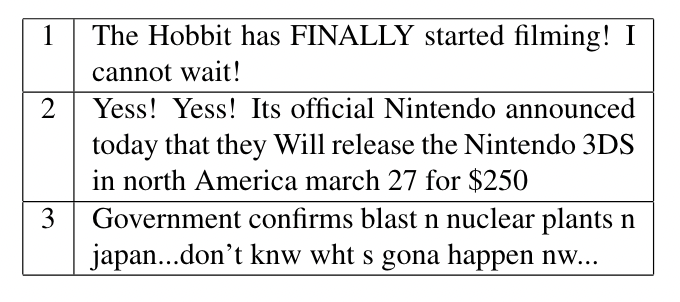
\includegraphics[keepaspectratio]{images/noisy_texts_ritter.png}  \caption{Examples of noisy text in tweets, taken from \cite{ritter_2011}}
  \label{fig:noisy_texts}
\end{figure}
 
Furthermore, since texts from social media are often \textbf{shorter of length}, they lack sufficient context for the determination of an entity's type (cf. \cite{ritter_2011}).

The \textbf{wide variety of capitalization styles} are another challenge, like e.g. the use of only lowercase for German texts, or the use of uppercase only in some texts (cf. \cite{ritter_2011}). As \cite{ritter_2011} point out, news-trained NER systems seem to rely heavily on capitalization which limits their applicability to user-generated social media texts. 

Also, these texts usually contain more \textbf{out of vocabulary (OOV) words} than e.g. news articles. This is partly due to misspellings, but also stems from platform specific codes and styles: The frequent occurence of \textbf{special characters} such as \# for hashtags or \@ for user mentions poses challenges because they cannot easily be handled during annotation and training. User-generated text in social media also often includes a lot of \textbf{lexical variations}. As an example, \cite{ritter_2011} collected more than fifty variations for the word `tomorrow' from a Twitter corpus, as shown in figure \ref{fig:lex_var}.

\begin{figure}[H]
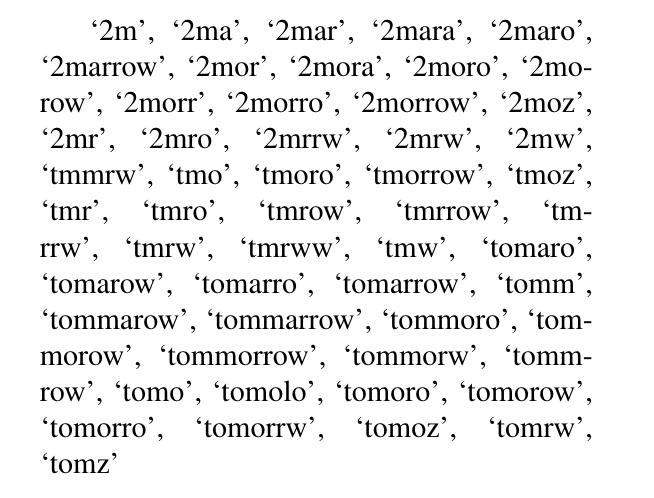
\includegraphics[keepaspectratio]{images/lexical_variations_ritter.png}  \caption{Lexical variations of the word `tomorrow' in tweets, taken from \cite{ritter_2011}}
  \label{fig:lex_var}
\end{figure}

Last but not least, social media texts often \textbf{mixed-language texts}, making it harder for language-specific models to accurately determine named entities in them. 

Named entity recognition applications for other domains thus usually require the creation of custom corpora including a labor-intensive annotation process, or rely on automatically generated annotations of large text corpora, often resulting in inconsistent annotations. 